\documentclass[tikz,dvisvgm,border=0pt]{standalone}
\usepackage{amssymb,amsmath}
\usetikzlibrary{positioning,fit,shapes.geometric,arrows.meta,calc}
\tikzset{every node/.append style={font=\huge}}
\makeatletter
% #1 = node name, #2 = extra CSS class (may be empty)
\newcommand{\hotspotX}[2]{%
  \path \pgfextra{\special{dvisvgm:raw <g class="hotspot #2" id="node-#1">}};
  \fill[white, fill opacity=0.01] (#1.north west) rectangle (#1.south east);
  \path \pgfextra{\special{dvisvgm:raw </g>}};}
\newcommand{\hotspot}[1]{\hotspotX{#1}{}}
\makeatother
\begin{document}
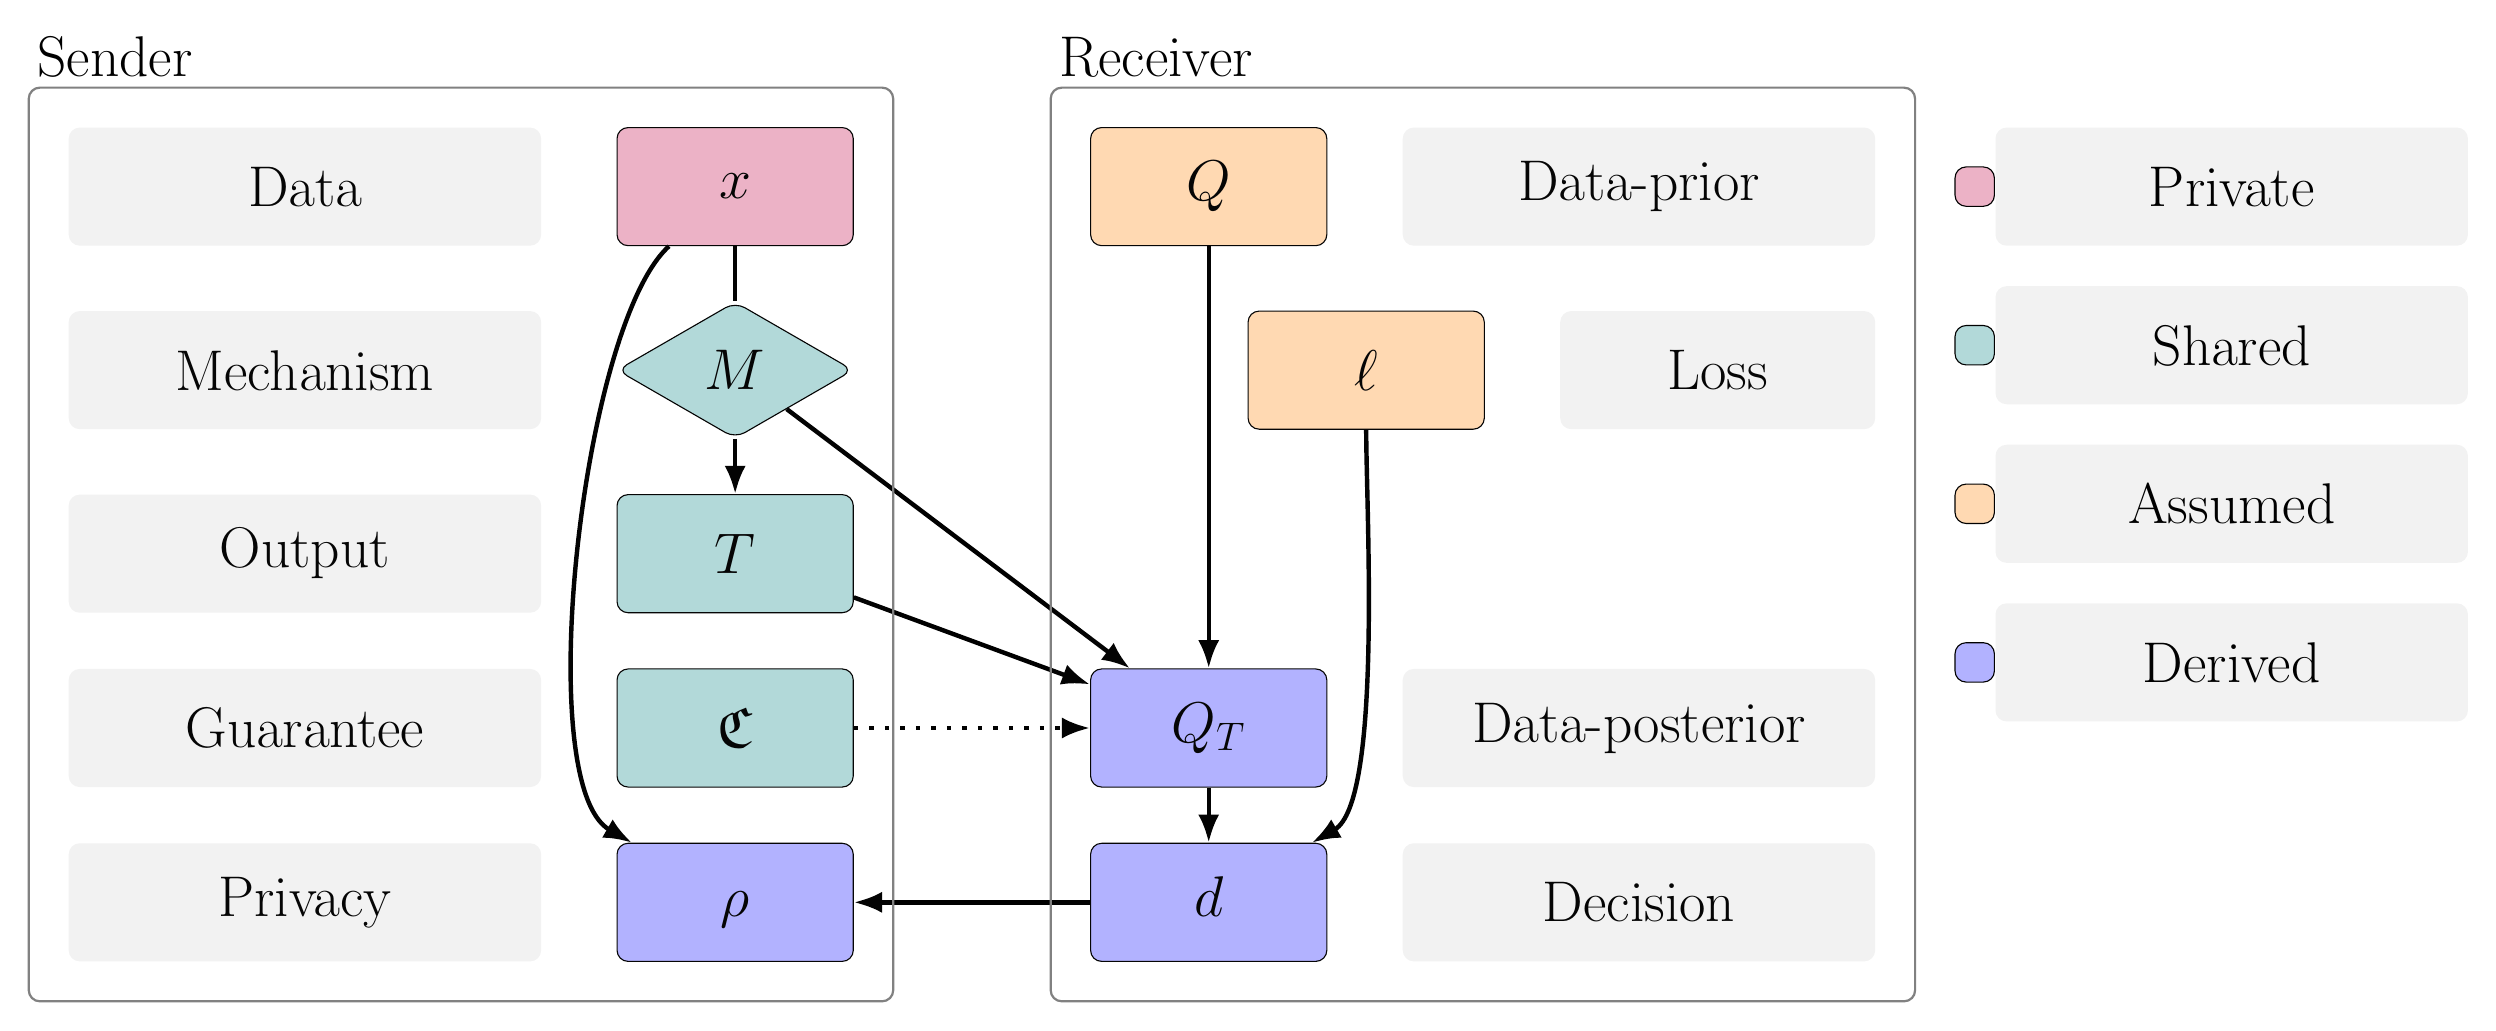
\begin{tikzpicture}
		\tikzstyle{privbox} = [rectangle, rounded corners, minimum width=3cm, minimum height=1.5cm, text centered, draw=black, fill=purple!30];
		\tikzstyle{inferbox} = [rectangle, rounded corners, minimum width=3cm, minimum height=1.5cm, text centered, draw=black, fill=blue!30];
		\tikzstyle{sharebox} = [rectangle, rounded corners, minimum width=3cm, minimum height=1.5cm,text centered, draw=black, fill=teal!30];
		\tikzstyle{shareboxmech} = [diamond, rounded corners, minimum width=3cm, minimum height=1cm,text centered, draw=black, fill=teal!30];
		\tikzstyle{desc} = [rectangle, minimum width=6cm, rounded corners, minimum height=1.5cm,text centered, fill=gray!10];
        \tikzstyle{desc2} = [rectangle, minimum width=4cm, rounded corners, minimum height=1.5cm,text centered, fill=gray!10];
		\tikzstyle{greybox} = [draw=gray, rounded corners, inner sep=0.5cm, thick];
		\tikzstyle{shareboxcolour} = [rectangle, rounded corners, minimum width=0.5cm, minimum height=0.5cm,text centered, draw=black, fill=teal!30];
		\tikzstyle{privboxcolour} = [rectangle, rounded corners, minimum width=0.5cm, minimum height=0.5cm,text centered, draw=black, fill=purple!30];
		\tikzstyle{modelboxcolour} = [rectangle, rounded corners, minimum width=0.5cm, minimum height=0.5cm,text centered, draw=black, fill=orange!30];
        \tikzstyle{modelbox} = [rectangle, rounded corners, minimum width=3cm, minimum height=1.5cm,text centered, draw=black, fill=orange!30];
        \tikzstyle{impliedboxcolour} = [rectangle, rounded corners, minimum width=0.5cm, minimum height=0.5cm,text centered, draw=black, fill=blue!30];
		\node (sdata) [privbox] {$x$};
		\node (sdatad) [desc, left=0.95cm of sdata] {Data};
		\node (mech) [shareboxmech, below=0.7cm of sdata] {$M$};
		\node (sstat) [sharebox, below=0.7cm of mech] {$T$};
		\node (strans) [sharebox, below=0.7cm of sstat] {$\mathfrak{C}$};
		\node (spriv) [inferbox, below=0.7cm of strans] {$\vphantom{d}\rho$};
		\node (sprivd) [desc, left=0.95cm of spriv] {Privacy};
		\node (adata) [modelbox, right=3cm of sdata] {$Q$};
		\node (adatad) [desc, right=0.95cm of adata] {Data-prior};
		\node (apost) [inferbox, right=3cm of strans] {$Q_T$};
		\node (aact) [inferbox, right=3cm of spriv] {$d\vphantom{\rho}$};
		\node (aactd) [desc, right=0.95cm of aact] {Decision};
		\node (aloss) [modelbox, right=5cm of mech] {$\ell$};
		\node (alossd) [desc2, right=0.95cm of aloss] {Loss};
		\node (private) [privboxcolour, right=1.5cm of adatad, xshift=-0.5cm] {};
		\node (privated) [desc, right=0pt of private] {Private};
		\node (public) [shareboxcolour, below=1.5cm of private] {};
		\node (publicd) [desc, right=0pt of public] {Shared};
		\node (modelled) [modelboxcolour, below=1.5cm of public] {};
		\node (modelledd) [desc, right=0pt of modelled] {Assumed};
        \node (implied) [impliedboxcolour, below=1.5cm of modelled] {};
		\node (impliedd) [desc, right=0pt of implied] {Derived};
		\draw[ultra thick, -] (sdata) -- (mech);
		\draw[ultra thick, -Latex] (mech) -- (sstat);
		\draw[ultra thick, -Latex] (sdata) to[out=222, in=150, looseness=0.5] (spriv);
		\draw[ultra thick, -Latex] (adata) -- (apost);
		\draw[ultra thick, -Latex] (apost) -- (aact);
		\draw[ultra thick, -Latex] (aloss) to[out=-90, in=30, looseness=0.5] (aact);
		\draw[ultra thick, -Latex] (mech) -- (apost);
		\draw[ultra thick, -Latex] (sstat) -- (apost);
		\draw[loosely dotted, ultra thick, -Latex] (strans) -- (apost);
		\draw[ultra thick, -Latex] (aact) -- (spriv);
        \node (apostd) [desc, right=0.95cm of apost] {Data-posterior};
        \node (mechd) [desc, left=0.95cm of mech] {Mechanism};
        \node (sstatd) [desc, left=0.95cm of sstat] {Output};
        \node (stransd) [desc, left=0.95cm of strans] {Guarantee};
		\node[greybox, fit=(sdata) (sdatad) (sstat) (sstatd) (strans) (stransd) (spriv) (sprivd) (mechd)] (statbox) {};
		\node[greybox, fit=(adata) (adatad) (apost) (apostd) (aact) (aactd) (aloss) (alossd)] (advbox) {};
		\node[anchor=south west, xshift=0cm] at (statbox.north west) {Sender};
		\node[anchor=south west, xshift=0cm] at (advbox.north west) {Receiver};
        % ===== interactive hotspot layer =====
        % Containers FIRST so they sit beneath the inner nodes (inner nodes win the pointer).
        \hotspotX{statbox}{container}\hotspotX{advbox}{container}
        % Inner content nodes + labels + legend (painted on top -> fully hoverable).
        \hotspot{sdata}\hotspot{mech}\hotspot{sstat}\hotspot{strans}\hotspot{spriv}
        \hotspot{adata}\hotspot{apost}\hotspot{aact}\hotspot{aloss}
        \hotspot{sdatad}\hotspot{mechd}\hotspot{sstatd}\hotspot{stransd}\hotspot{sprivd}
        \hotspot{adatad}\hotspot{apostd}\hotspot{aactd}\hotspot{alossd}
	\end{tikzpicture}
\end{document}
